\documentclass{beamer}

\newcommand{\week}{Equities-3}

\title{Equity Valuation}
\subtitle{Reference: Bodie et al, Ch 18}
\author{Econ 457}
\date{\week}

% Reference the shared preamble
\setbeamertemplate{frametitle}{
  \vspace{0.5em}
  \insertframetitle
  \par
  \vspace{0.5em}
  \hrule
  \vspace{0.3em}
  {\small\color{gray}\insertframesubtitle}
}

\setbeamertemplate{navigation symbols}{}
\setbeamertemplate{itemize item}{\textbullet} % main bullet: filled dot
\setbeamertemplate{itemize subitem}{\normalsize$\circ$} % sub-bullet: empty dot
\setbeamertemplate{itemize subsubitem}{\scriptsize--} % sub-sub-bullet: dash


% Font changes
\usepackage[scaled=0.92]{helvet}
\renewcommand{\familydefault}{\sfdefault}

% Packages
\usepackage{tikz}
\usepackage{booktabs}
\usepackage{xcolor}
\usepackage{array}           % Enhanced column types for tables
\usepackage{multirow}        % Spanning multiple rows in tables
\usepackage{makecell}        % Line breaks and formatting in table cells
\usepackage{siunitx}         % Proper formatting of numbers and units
\usepackage{amsmath}         % Enhanced math environments
\usepackage{amsfonts}        % Additional math fonts
\usepackage{amssymb}         % Additional math symbols
\usepackage{url}             % Better URL formatting
\usepackage{graphicx}        % Enhanced graphics support
\usepackage{tabularray}
\UseTblrLibrary{booktabs, siunitx, varwidth}
% For financial presentations specifically
\usepackage{eurosym}         % Euro symbol
\usepackage{textcomp}        % Additional text symbols
\usepackage{hyperref}        % Hyperlinks (should be loaded last)

% Define a footnote
\renewcommand{\footnoterule}{\vspace*{-3pt}\hrule width 2in height 0.4pt\vspace*{2.6pt}}

% Define a Foundation Slide
\newenvironment{foundframe}[1][t]{
    \setbeamercolor{background canvas}{bg=gray!8}
    \setbeamercolor{frametitle}{fg=gray!80!black,bg=gray!25}
    \setbeamercolor{framesubtitle}{fg=gray!70!black,bg=gray!15}
    \setbeamercolor{item}{fg=gray!80!black}
    \setbeamercolor{enumerate item}{fg=gray!80!black}
    
    % Modify the frametitle template for this frame type
    \setbeamertemplate{frametitle}{
        \vspace{0.5em}
        \begin{minipage}[t]{0.75\textwidth}
            \insertframetitle
            \par
            \vspace{0.5em}
            \hrule
            \vspace{0.3em}
            {\small\color{gray}\insertframesubtitle}
        \end{minipage}%
        \hfill
        \begin{minipage}[t]{0.2\textwidth}
            \raggedleft
            \colorbox{gray!30}{%
                \scriptsize\bfseries\color{gray!80!black}%
                   \hspace{3pt}\begin{tabular}{c}Foundation\\Material\end{tabular}\hspace{3pt}%
            }
        \end{minipage}
        \vspace{0.3em}
    }
    
    \begin{frame}[#1]
}{
    \end{frame}
}

% Define Practice Slide
\newenvironment{practiceframe}[1][t]{
    \setbeamercolor{background canvas}{bg=white}
    \setbeamercolor{frametitle}{fg=blue!80!black,bg=blue!15}
    \setbeamercolor{framesubtitle}{fg=blue!70!black,bg=blue!10}
    \setbeamercolor{item}{fg=blue!80!black}
    \setbeamercolor{enumerate item}{fg=blue!80!black}
    \setbeamercolor{normal text}{fg=blue!90!black}
    
    % Modify the frametitle template for this frame type
    \setbeamertemplate{frametitle}{
        \vspace{0.5em}
        \begin{minipage}[t]{0.75\textwidth}
            \insertframetitle
            \par
            \vspace{0.5em}
            \hrule
            \vspace{0.3em}
            {\small\color{blue!70!black}\insertframesubtitle}
        \end{minipage}%
        \hfill
        \begin{minipage}[t]{0.2\textwidth}
            \raggedleft
            \colorbox{blue!20}{%
                \scriptsize\bfseries\color{blue!80!black}%
                   \hspace{3pt}\begin{tabular}{c}Practice\\Questions\end{tabular}\hspace{3pt}%
            }
        \end{minipage}
        \vspace{0.3em}
    }
    
    \begin{frame}[#1]
}{
    \end{frame}
}

% Define Excel Slide
\newenvironment{excelframe}[1][t]{
    \setbeamercolor{background canvas}{bg=white}
    \setbeamercolor{frametitle}{fg=blue!80!black,bg=blue!15}
    \setbeamercolor{framesubtitle}{fg=blue!70!black,bg=blue!10}
    \setbeamercolor{item}{fg=blue!80!black}
    \setbeamercolor{enumerate item}{fg=blue!80!black}
    \setbeamercolor{normal text}{fg=blue!90!black}
    
    % Modify the frametitle template for this frame type
    \setbeamertemplate{frametitle}{
        \vspace{0.5em}
        \begin{minipage}[t]{0.75\textwidth}
            \insertframetitle
            \par
            \vspace{0.5em}
            \hrule
            \vspace{0.3em}
            {\small\color{blue!70!black}\insertframesubtitle}
        \end{minipage}%
        \hfill
        \begin{minipage}[t]{0.2\textwidth}
            \raggedleft
            \colorbox{green!10}{%
                \scriptsize\bfseries\color{blue!80!black}%
                   \hspace{3pt}\begin{tabular}{c}MS Excel\end{tabular}\hspace{3pt}%
            }
        \end{minipage}
        \vspace{0.3em}
    }
    
    \begin{frame}[#1]
}{
    \end{frame}
}

% Define Caution Slide
\newenvironment{cautionframe}[1][t]{
    \setbeamercolor{background canvas}{bg=white}
    \setbeamercolor{frametitle}{fg=blue!80!black,bg=blue!15}
    \setbeamercolor{framesubtitle}{fg=blue!70!black,bg=blue!10}
    \setbeamercolor{item}{fg=blue!80!black}
    \setbeamercolor{enumerate item}{fg=blue!80!black}
    \setbeamercolor{normal text}{fg=blue!90!black}
    
    % Modify the frametitle template for this frame type
    \setbeamertemplate{frametitle}{
        \vspace{0.5em}
        \begin{minipage}[t]{0.75\textwidth}
            \insertframetitle
            \par
            \vspace{0.5em}
            \hrule
            \vspace{0.3em}
            {\small\color{blue!70!black}\insertframesubtitle}
        \end{minipage}%
        \hfill
        \begin{minipage}[t]{0.2\textwidth}
            \raggedleft
            \colorbox{red!10}{%
                \scriptsize\bfseries\color{blue!80!black}%
                   \hspace{3pt}\begin{tabular}{c}Caution\end{tabular}\hspace{3pt}%
            }
        \end{minipage}
        \vspace{0.3em}
    }
    
    \begin{frame}[#1]
}{
    \end{frame}
}

% Add to footnotes
\makeatletter
\newcommand\blfootnote[1]{%
  \begingroup
  \renewcommand\thefootnote{}%
  \renewcommand\@makefntext[1]{\raggedright\leftskip=0pt ##1}%
  \footnote{\scriptsize #1}%
  \addtocounter{footnote}{-1}%
  \endgroup
}
\makeatother

% Quote Command
% Preamble
\newcommand{\myquote}[2]{%
  \par\begingroup
  \begin{center}
    \begin{minipage}{0.8\textwidth} % adjust width here
      \itshape
      #1\par
      \medskip
      \begin{flushright}
        \normalfont\small #2
      \end{flushright}
    \end{minipage}
  \end{center}
  \endgroup
}

% Set the footer -- change 
\setbeamertemplate{footline}{
  \leavevmode%
  \vspace{2ex}
  \hbox{%
    % Left box: Econ 457
    \begin{beamercolorbox}[wd=.4\paperwidth,ht=2.5ex,dp=1ex,left]{author in head/foot}%
      \hspace{1em}Econ 457
    \end{beamercolorbox}%
    % Middle box: Week
    \begin{beamercolorbox}[wd=.2\paperwidth,ht=2.5ex,dp=1ex,center]{date in head/foot}%
      \centering\week
    \end{beamercolorbox}%
    % Right box: Slide numbers
    \begin{beamercolorbox}[wd=.4\paperwidth,ht=2.5ex,dp=1ex,center]{date in head/foot}%
      \hfill\insertframenumber{} 
    \end{beamercolorbox}%
  }%
  \vskip0pt%
}

\begin{document}

\frame{\titlepage}

\begin{frame}
    \frametitle{Outline}

    \begin{enumerate}
        \item Relative Valuation 
        \item Growth and the P/E Ratio
        \item Uses of the P/E Ratio
        \item Cyclically Adjusted P/E (CAPE)
    \end{enumerate}

\end{frame}

\begin{frame}[t]
    \frametitle{1. Relative Valuation}
    \section{P/E Ratio}

    Question: Consider a company that expects to earn \$100 billion in the coming year. Assume the company has no debt and pays all its earning to shareholders via dividends.
    
    \vspace{1em}
    How much would you pay to own the entire company? Why?
    \begin{enumerate}[(A)]
        \item \$100 billion
        \item More than \$100 billion
        \item Less than \$100 billion
        \item No idea
    \end{enumerate}
    \vspace{1em}
    \blfootnote{Hint: think about the Gordon Growth Model}

\end{frame}

\begin{frame}[t]
    \frametitle{1. Relative Valuation}
    \framesubtitle{P/E Ratio}

    The value of a perpetuity is given by:
    $$P_0 = \frac{c}{k}$$
    Where $P_0$ is the current price, $c$ is the payment amount, and $k$ is the discount rate.\\
    \vspace{1em}
    If a company pays all of its earnings out as dividends ($D_i=E_i$ for all $i$), then it will have no growth.  The value of that company will be a perpetuity.\\
    $$P_0 = \frac{E}{k}$$

    \blfootnote{The expression for a perpetuity comes from the same infinite series trick we used to derive the Gordon Growth Model.  Alternatively, you can use the Gordon Growth model and set $g=0$}
        
\end{frame}

\begin{frame}[t]
    \frametitle{1. Relative Valuation}
    \framesubtitle{P/E Ratio}

    Define the \textbf{Price-Earnings Ratio} as $P/E$ where $P$ is the market price of the company and $E$ is its earnings.  For a company with no growth, earnings in the denominator and numerator cancel and this becomes:
    $$P_0/E = \frac{1}{k}$$
    \vspace{1em}
    
    For illustrative purposes, assume that $k=12.5\%$. When the P-E Ratio would be $1/0.125 = 8$.
    \vspace{1em}

    In words: investors should be willing to pay \$8 billion for a company with a 
    required return of 12.5\%, no-growth prospects, and earnings next year of \$1 billion.

\end{frame}

\begin{frame}[t]
    \frametitle{1. Relative Valuation}
    \framesubtitle{P/E Ratio}

    Of course, companies also have growth prospects, which should increase their value.  
    We can define the value of a company as follows:
    \begin{align*}
    P_0 &= \text{PV(no-growth)} + \text{PV(Growth Opportunities)}\\
        &= \frac{E_1}{k} + PVGO
    \end{align*}
    Where $PVGO$ is $PV(Growth Opportunities)$\\

\end{frame}

\begin{frame}[t]
    \frametitle{1. Relative Valuation}
    \framesubtitle{P/E Ratio}

    Dividing this by $E_1$ and doing a little rearranging 
    gives an expression for the P/E Ratio:
    $$
    \frac{P_0}{E_1} = \frac{1}{k} \left(1 + \frac{PVGO}{E/k}\right)
    $$
    The term $\frac{PVGO}{E/k}$ is the ratio of the growth opportunities 
    to the no-growth scenario for the firm.  And the term $\frac{1}{k}$ is 
    what we say earlier about the PE ratio for a no-growth firm.\\
    \vspace{1em}
    In words, the PE ratio is the value of a perpetuity multiplied by 
    one plus the ratio of PVGO to the no-growth value.  Firms will higher 
    PVGOs will have higher PE ratios.   Investors are willing to pay more 
    for companies with better growth prospects.

\end{frame}


\begin{frame}[t]
    \frametitle{1. Relative Valuation}
    \framesubtitle{P/E Ratio - Earnings}

        To calculate a P/E ratio, we need a measure of earnings.
        
        \vspace{1em}
        
        \begin{itemize}
            \item \textbf{Forward P/E}: Uses expected earnings over the next
            12 months. Estimates may come from company guidance, analyst
            consensus forecasts, or your own analysis.
        
            \item \textbf{Trailing P/E}: Uses actual earnings over the
            trailing twelve months (TTM). These are readily available
            and do not require forecasts, but may not reflect future
            earnings.
        \end{itemize}
        
        \vspace{1em}
        
        Forward earnings are generally more relevant for valuation,
        but they introduce uncertainty because they rely on forecasts.

\end{frame}

\begin{frame}[t]
    \frametitle{1. Relative Valuation}
    \framesubtitle{Per Share vs. Total Equity Value}

    The P/E ratio can be calculated using either the price
    and earnings per share, or the value and earnings of
    the entire company.

    {\footnotesize
    \begin{align*}
    EPS &= \frac{\text{Net Income}}{\text{Shares Outstanding}}\\
    \text{Equity Value} &= \text{Price per Share} \times \text{Shares Outstanding}\\
    \end{align*}}

    Therefore:
    {\footnotesize
    \begin{align*}
        P/E &= \frac{\text{Price per Share}}{EPS}\\
            &= \frac{\text{Price per Share}}
            {\frac{\text{Net Income}}{\text{Shares Outstanding}}}\\
            &= \frac{\text{Price per Share}\times
            \text{Shares Outstanding}}{\text{Net Income}} = \boxed{\frac{\text{Equity Value}}{\text{Net Income}}}
    \end{align*}}

    The two approaches are equivalent because the number of
    shares outstanding cancels out.

\end{frame}

\begin{practiceframe}[t]
\frametitle{1. Relative Valuation}
\framesubtitle{Growth and PE Ratio}

    \begin{enumerate}
        \item Computer stocks current provide an expected rate of return 
        of 16\%.   MBI, a large computer company will pay a year-end dividend of \$2 
        per share.   If the stock is selling at \$50 per share, what must be the market's 
        expectation for the dividend growth rate?
        \begin{enumerate}
        \item[a. ] If the dividend growth forecast is revised down to 5\%, what will have to the price of stock?  What (qualitatively) will happen to the price-earnings ratio?
        \end{enumerate}
        \item The FI Corporation's dividends per share are expected to 
        grow indefinitely by 5\% per year.  If this year's year-end dividend is \$8 and the market capitalization rate is 10\% per year, what must be the current stock price? If the expected earnings per share are \$12, what is the implied value of the ROE on future investment opportunities?   How much is the market paying per share for future growth?  What is the PE Ratio?
    \end{enumerate}

\end{practiceframe}

\begin{frame}[t]
    \frametitle{2. Growth and the P/E ratio}
    \section{Growth and the P/E Ratio}

    \begin{itemize}
        \item The price of stocks (and the P/E ratio) necessarily require forecasts for future growth.
        \item Specifically, companies with high P/E ratios are generally expected to have high growth rates
        \begin{itemize} 
            \item Theoretically high P/E ratios could also be due to low discount rates, but usually growth rates are the more important driver.
        \end{itemize}
        \item As the next example shows, sometimes markets and investors get it right, sometimes they don't.
    \end{itemize}

\end{frame}

\begin{frame}[t]
    \frametitle{2. Growth and the P/E ratio}

    \textbf{Software and Chip (Semiconductor) PE Ratios in January 2025}
        \begin{itemize}
        \item At the beginning of 2025, software and semiconductor sectors both had very high forward PE ratios (above 50).
        \item These high PE ratios corresponded with very high growth expectations (above 20\% for five years)
    \end{itemize}

\end{frame}

\begin{frame}[t]
    \frametitle{2. Growth and the P/E ratio}

    \centering
    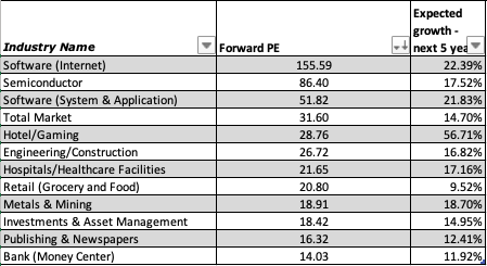
\includegraphics[width=0.9\textwidth]{Econ357/figures/02_mkts_7_damadoaran.png}

    \blfootnote{Source: Aswath Damodaran's website, January 2025}

\end{frame}

% https://pages.stern.nyu.edu/~adamodar/New_Home_Page/datafile/pedata.html

\begin{frame}[t]
    \frametitle{2. Growth and the P/E ratio}
    \framesubtitle{NVDA}

    \begin{itemize}
        \item Nvidia (NVDA) had an extremely high PE in 2023.
        \item NVDA earnings growth has been astounding since.  
        \item NVDA price has continued to increase, although the PE ratio has come down.
    \end{itemize}
    \vspace{1em}

    \centering
    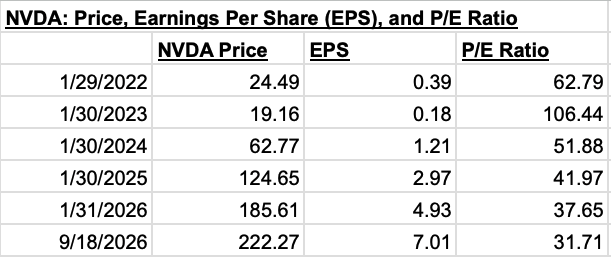
\includegraphics[width=0.8\textwidth]{Econ357/figures/02_mkts_7_nvda.png}

    \blfootnote{Source: Marketwatch, Google Finance}

\end{frame}

% https://docs.google.com/spreadsheets/d/18M0LUbKakHxFRbQy0rqCKJI-eFjZkZu4SkjLEp2maCA/edit?gid=1620244217#gid=1620244217

\begin{frame}[t]
    \frametitle{2. Growth and the P/E ratio}
    \framesubtitle{ADBE}

    \begin{itemize}
        \item Software stocks had high PEs at the beginning of 2025.
        \item Since then, EPS for ADBE has continued to grow.
        \item Future growth expectations have come down, however, and so has the P/E ratio.
    \end{itemize}

    \centering
    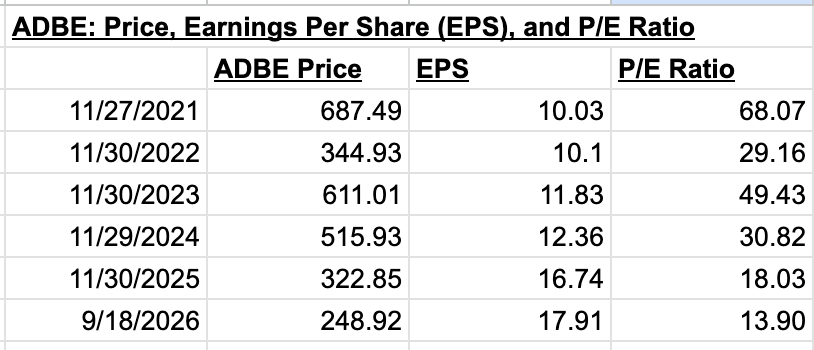
\includegraphics[width=0.8\textwidth]{Econ357/figures/02_mkts_adbe.png}

    \blfootnote{Source: Marketwatch, Google Finance}

\end{frame}

\begin{frame}[t]
    \frametitle{2. Growth and the P/E ratio}
    \framesubtitle{NVDA v ADBE}

    \centering
    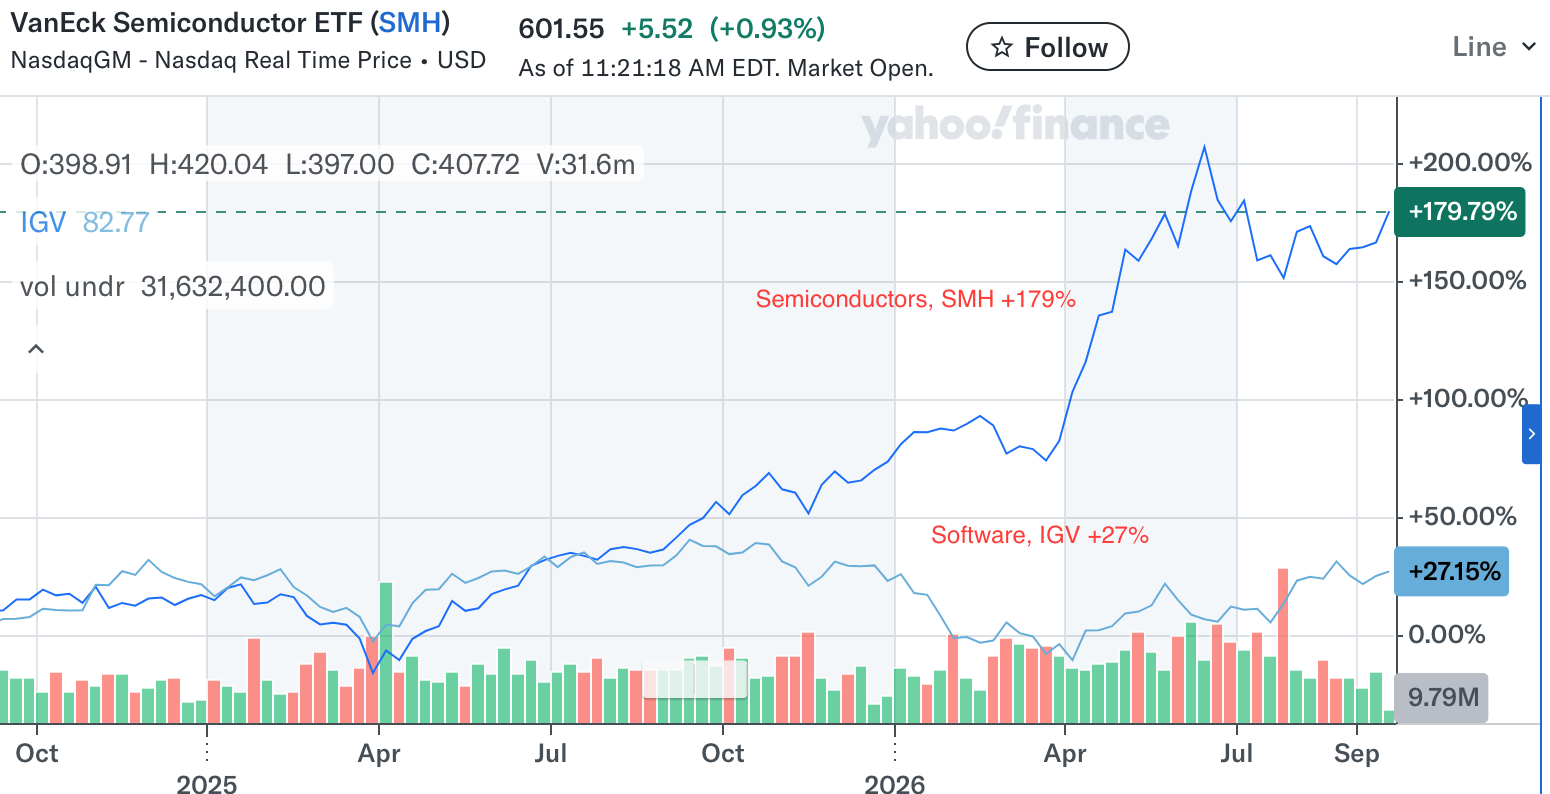
\includegraphics[width=\textwidth]{Econ357/figures/02_mkts_igv.png}

    \blfootnote{Source: Yahoo Finance}

\end{frame}


% https://www.wsj.com/market-data/stocks/peyields?mod=md_usstk_view_pe_yield_full

\begin{frame}[t]
    \frametitle{3. Uses of the P/E ratio}
    \section{Uses of the P/E Ratio}

    In contrast to the Gordon Growth Model, which we used to estimate the value of company, the P/E ratio is used to make \textit{relative} statements about prices.   
    \vspace{1em}
    
    In particular, P/E ratios are often used to:
    \begin{enumerate}
        \item Compare the prices of similar companies
        \item Price IPOs or acquisitions
    \end{enumerate}
    \vspace{1em}
   

\end{frame}



\begin{frame}[t]
    \frametitle{3. Uses of the P/E ratio}
    \framesubtitle{Comparing Prices of Similar Companies}

    % Requires: \usepackage{booktabs}
    \begin{table}[h]
        \caption{Bank PE Ratios, Sep 2026}
        \label{tab:placeholder_label}
        \centering
        \begin{tabular}{lrr}
            \toprule
            Company & P/E (TTM) \\
            \midrule
            JPMorgan Chase \& Co. & 14.98 \\
            Bank of America Corp.  & 13.29 \\
            Wells Fargo \& Co. & 12.51 \\
            Royal Bank of Canada  & 17.94 \\
            Toronto-Dominion Bank  & 18.39 \\
            Citigroup Inc. & 14.22 \\
            HSBC Holdings PLC  & 14.53 \\
            BNP Paribas S.A.  & 8.72 \\
            \bottomrule
        \end{tabular}
    \end{table}

    \blfootnote{Source: Wall Street Journal, September 2026}

\end{frame}

% https://www.wsj.com/market-data/quotes/US/XNYS/JPM

\begin{frame}[t]
    \frametitle{3. Uses of the P/E ratio}
    \framesubtitle{Comparing Prices of Similar Companies}

    % Requires: \usepackage{booktabs}
    \begin{table}[h]
        \centering
        \caption{Automaker PE Ratios, July 2025}
        \begin{tabular}{lrrrr}
            \toprule
            & \multicolumn{1}{c}{\begin{tabular}[c]{@{}c@{}}Market\\ Cap\\ \$ bn\end{tabular}} &
            \multicolumn{1}{c}{\begin{tabular}[c]{@{}c@{}}Share Price, \$\\ (as of 7-16)\end{tabular}} &
            \multicolumn{1}{c}{\begin{tabular}[c]{@{}c@{}}EPS,\\ TTM\end{tabular}} &
            \multicolumn{1}{c}{\begin{tabular}[c]{@{}c@{}}PE Ratio,\\ TTM\end{tabular}} \\
            \midrule
            Ford (F)            & 44.6  & 11.25  & 1.25 & 9.00  \\
            General Motors (GM) & 51.1  & 53.33  & 7.16 & 7.45  \\
            Honda (HMC)         & 41.8  & 30.53  & 3.64 & 8.39  \\
            Tesla (TSLA)        & 1{,}037 & 321.88 & 1.74 & \textbf{184.99} \\
            BYD Company (BYD)   & 172.6 & 93.73  & 4.30 & 21.77 \\
            \bottomrule
        \end{tabular}
    \end{table}

    \blfootnote{Data from Yahoo Finance, as of 7-16-2025}

\end{frame}

\begin{frame}[t]
\frametitle{3. Uses of the P/E ratio}

The P/E ratio can be used to estimate the value of a company:

\[
P/E=\frac{\text{Price}}{\text{Earnings}}
\]

\begin{itemize}
    \item Use the P/E ratios of comparable companies to select an
    appropriate multiple.

    \item For an IPO:
    \[
    \text{Implied Price}
    =
    \text{P/E Multiple}\times\text{EPS}.
    \]


    \item The appropriate multiple depends on factors such as growth,
    risk, and etc.
    \item \textbf{Example}: Jersey Mike's did an IPO in 2026.   The P/E ratio on their IPO was around 30x.
\end{itemize}

\end{frame}

\begin{frame}[t]
    \frametitle{4. CAPE}
    \section{CAPE}
    \framesubtitle{Comparing Prices Across Time}

    \textbf{Cyclically Adjusted PE Ratio ("CAPE")}
    \begin{itemize}
        \item Created by Robert Shiller (Yale Professor, Nobel Prize 2013)
        \item Today's price divided by average earnings over the past 10 years (both adjusted for inflation)
        \item Data available back to 1880 
        \item Advantage: smooths out business cycles (e.g. 2008)
        \item Disadvantage: some prefer to use \textit{forward} earnings
    \end{itemize}
\end{frame}

\begin{frame}[t]
    \frametitle{4. CAPE}
    \framesubtitle{Comparing Prices Across Time}

    \centering
    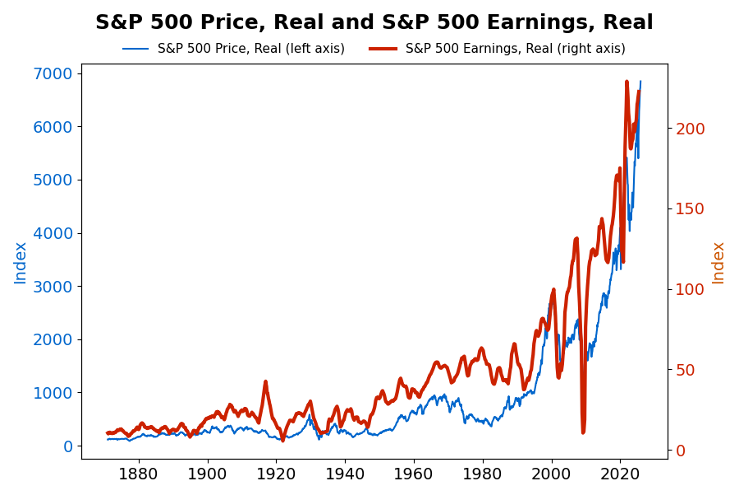
\includegraphics[width=0.9\textwidth]{Econ357/figures/02_mkts_7_shiller1.png}

\end{frame}

\begin{frame}[t]
    \frametitle{3. Uses of the P/E ratio}
    \framesubtitle{Comparing Prices Across Time}

    \centering
    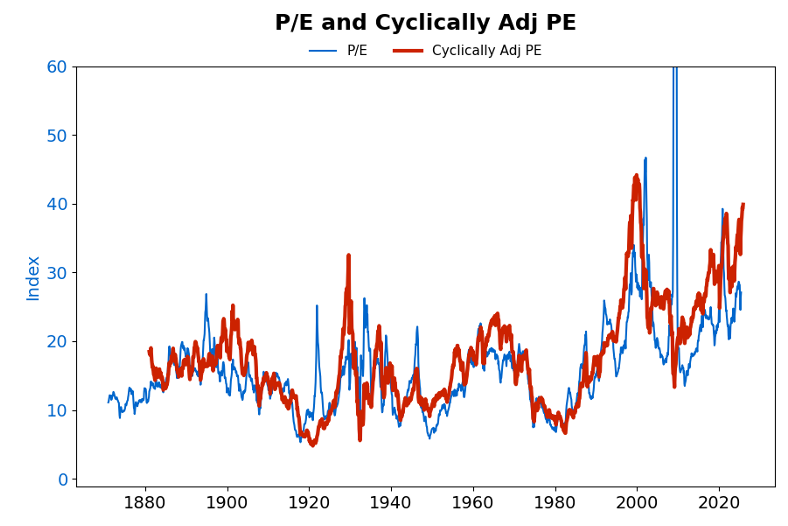
\includegraphics[width=0.9\textwidth]{Econ357/figures/02_mkts_7_shiller2.png}

\end{frame}

\begin{frame}[t]
    \frametitle{4. CAPE}
    \framesubtitle{Comparing Prices Across Time}

    Is the CAPE a useful signal for when stocks are expensive or cheap?
    
    \vspace{1em}
    The inverse of the CAPE is the 'earnings yield'.   This could plausibly correspond with the expected earnings in the future, normalized by the price.     
    
    \vspace{1em}
    (Remember that we thought about bond yields as an indicator of expected of returns.  However, in bonds the final price is fixed at the face value, whereas there is no analogous final price in equities.)

\end{frame}

\begin{frame}[t]
    \frametitle{4. CAPE}
    \framesubtitle{Comparing Prices Across Time}

    \centering
    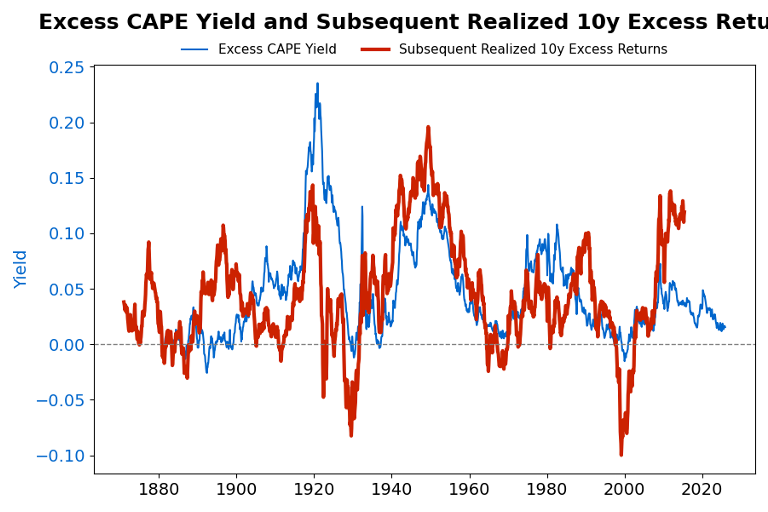
\includegraphics[width=0.9\textwidth]{Econ357/figures/02_mkts_7_shiller3.png}

\end{frame}


\begin{frame}[t]
    \frametitle{4. Cyclically Adjusted P/E (CAPE)}
    \framesubtitle{Barclays}

    \centering
    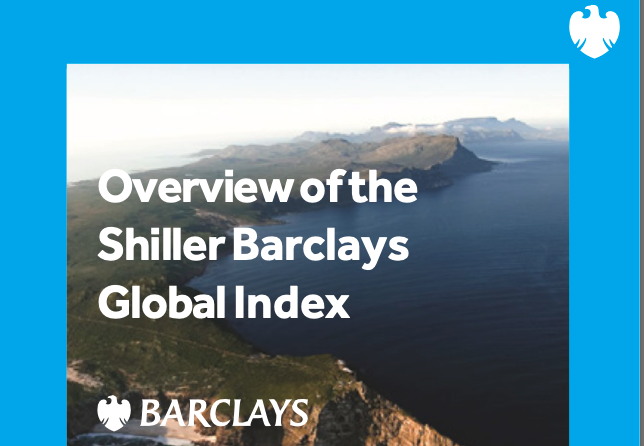
\includegraphics[width=0.8\textwidth]{figures/ch18_2_barclays.png}

\end{frame}

\begin{frame}[t]
    \frametitle{4. Cyclically Adjusted P/E (CAPE)}
    \framesubtitle{Barclays}

    \centering
    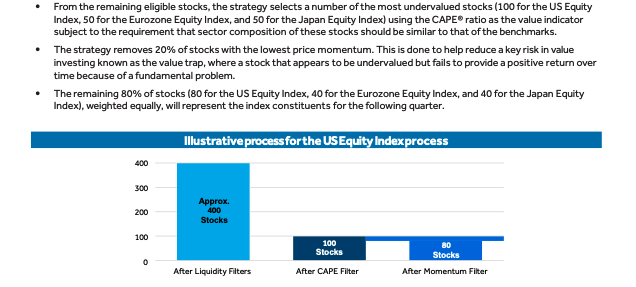
\includegraphics[width=\textwidth]{figures/ch18_2_barclays2.png}

\end{frame}





\end{document}